\section{Arquitectura Digital, Firmware Embebido y Plataforma IoT}

\subsection{Visión General de la Pila Tecnológica (Tres Capas Desacopladas)}
Para transformar las ecuaciones de control en un sistema físico supervisable y operable de forma remota, diseñé e implementé una arquitectura desacoplada en tres capas independientes:

\begin{figure}[htbp]
    \centering
    \resizebox{0.95\linewidth}{!}{
    \begin{tikzpicture}[
        layer/.style={rectangle, draw=black, fill=black!3, thick, rounded corners=1pt, minimum width=12cm, minimum height=1.2cm, align=left, font=\small},
        arrow/.style={-{Latex[length=2.5mm]}, thick, draw=black}
    ]
        % Capas centradas verticalmente
        \node [layer] (l3) at (0, 4.4) {\textbf{Capa 3: Interfaz de Usuario (Frontend Web)}\\Dashboard Reactivo en Astro + TypeScript + Apache ECharts + TailwindCSS (Puerto 4321 / 8080)};
        \node [layer] (l2) at (0, 2.2) {\textbf{Capa 2: Servidor Backend y Lazo de Control (Python)}\\API REST Flask + Hilo Serial Asíncrono a 115200 baud + Buffer Circular + Anti-Windup (Puerto 5000)};
        \node [layer] (l1) at (0, 0.0) {\textbf{Capa 1: Hardware y Firmware Embebido (ESP32 / C++)}\\Adquisición OneWire (DS18B20 en D15/D13) + Timer PWM LEDC (D25) + Servo (D27)};
        
        % Canal de Subida (Izquierda, x = -3.2 cm)
        \draw [arrow] (-3.2, 0.6) -- node[left, font=\footnotesize, align=right] {Telemetría Serial\\(115200 baud)} (-3.2, 1.6);
        \draw [arrow] (-3.2, 2.8) -- node[left, font=\footnotesize, align=right] {Telemetría JSON\\HTTP / Polling} (-3.2, 3.8);

        % Canal de Bajada (Derecha, x = +3.2 cm)
        \draw [arrow] (3.2, 3.8) -- node[right, font=\footnotesize, align=left] {Consignas y\\Setpoints de Control} (3.2, 2.8);
        \draw [arrow] (3.2, 1.6) -- node[right, font=\footnotesize, align=left] {Comandos PWM y\\Ángulo de Servomotor} (3.2, 0.6);
    \end{tikzpicture}
    }
    \caption{Arquitectura desacoplada en 3 capas desarrollada para ALUNA PBR-02.}
    \label{fig:arquitectura_iot}
\end{figure}

\subsection{Capa 1: Firmware Embebido en C++ para ESP32}
El firmware (\texttt{esp32\_firmware.ino}) fue programado desde cero en el entorno de Arduino Core para ESP32, optimizando los tiempos de ciclo y evitando cualquier bloqueo mediante temporización por milisegundos (\texttt{millis()}):

\begin{enumerate}[label=\textbf{\alph*.}]
    \item \textbf{Gestión del Bus 1-Wire y Resolución de Sensores:}
    Para garantizar máxima precisión sin introducir retardos inaceptables, configuré los sensores DS18B20 en una resolución de \textbf{10 bits} ($0.25\,^\circ\text{C}$ de resolución y tiempo de conversión de solo $187.5\,\text{ms}$, en contraste con los $750\,\text{ms}$ de la resolución de 12 bits):
    \begin{lstlisting}[language=C++]
// Configuracion de resolucion y conversion no bloqueante
sensorAgua15.setWaitForConversion(true);
sensorAire13.setWaitForConversion(true);
sensorAgua15.setResolution(10); // 187.5 ms tiempo de lectura
sensorAire13.setResolution(10);
    \end{lstlisting}

    \item \textbf{Generación de Señal PWM por Hardware en Pin D25:}
    En lugar de emular el PWM por software (lo que generaría \textit{jitter} y calentamiento por pérdidas de conmutación), configuré el periférico interno \textbf{LEDC} de la ESP32 a una frecuencia de \textbf{$1000\,\text{Hz}$ con resolución de 8 bits} ($0$ a $255$):
    \begin{lstlisting}[language=C++]
const int PELTIER_PWM_PIN = 25;
pinMode(PELTIER_PWM_PIN, OUTPUT);
ledcAttach(PELTIER_PWM_PIN, 1000, 8); // 1 kHz, 8 bits (0 - 255)
ledcWrite(PELTIER_PWM_PIN, pwm_actual);
    \end{lstlisting}

    \item \textbf{Control de Posición Angular del Servomotor en Pin D27:}
    Mediante la librería \texttt{ESP32Servo}, configuré el servomotor MG996R a una frecuencia base de $50\,\text{Hz}$ y anchos de pulso calibrados entre $500\,\mu\text{s}$ ($0^\circ$, abierto) y $2500\,\mu\text{s}$ ($180^\circ$, cerrado):
    \begin{lstlisting}[language=C++]
servoCortina.setPeriodHertz(50);
servoCortina.attach(SERVO_PIN, 500, 2500);
servoCortina.write(angulo_deseado); // 0 a 180 grados
    \end{lstlisting}
\end{enumerate}

\subsection{Capa 2: Servidor Backend y Lazo de Control Digital en Python}
El backend (\texttt{app.py}) fue desarrollado en Python utilizando Flask y multithreading:
\begin{itemize}
    \item \textbf{Hilo de Adquisición Asíncrona:} Un hilo demonio (\textit{daemon thread}) dedicado lee continuamente el puerto serial (\texttt{/dev/ttyUSB0}) a 115200 baud, decodifica los paquetes JSON emitidos por la ESP32 y filtra lecturas espurias (por ejemplo, el valor de error $-127.0\,^\circ\text{C}$ típico de desconexiones 1-Wire).
    \item \textbf{Buffer Circular en Memoria:} Almacena un historial deslizante de las últimas 3600 muestras (equivalente a 1 hora a $1\,\text{Hz}$), permitiendo entregar datos inmediatos al frontend sin saturar bases de datos en disco.
    \item \textbf{Lazo PI Cohen-Coon con Anti-Windup Digital:} Calcula el error de seguimiento $e_k = T_{\text{agua}} - T_{\text{setpoint}}$ y satura la acción integral mediante la técnica de \textit{clamping}:
    \begin{equation}
        u_k = K_p e_k + K_i \sum_{j=0}^{k} e_j \Delta t, \quad \text{con } u_k \in [0, 255]
    \end{equation}
    Si la salida $u_k$ se satura en 255 (100\% PWM) o en 0, la suma integral se congela para evitar el desbordamiento integral (\textit{integrator windup}) cuando el sistema enfrenta una perturbación térmica severa.
\end{itemize}

\subsection{Capa 3: Dashboard Web en Tiempo Real (Astro + ECharts)}
Diseñé el panel de control web priorizando la usabilidad operativa para evaluadores técnicos y biólogos.

\begin{figure}[htbp]
    \centering
    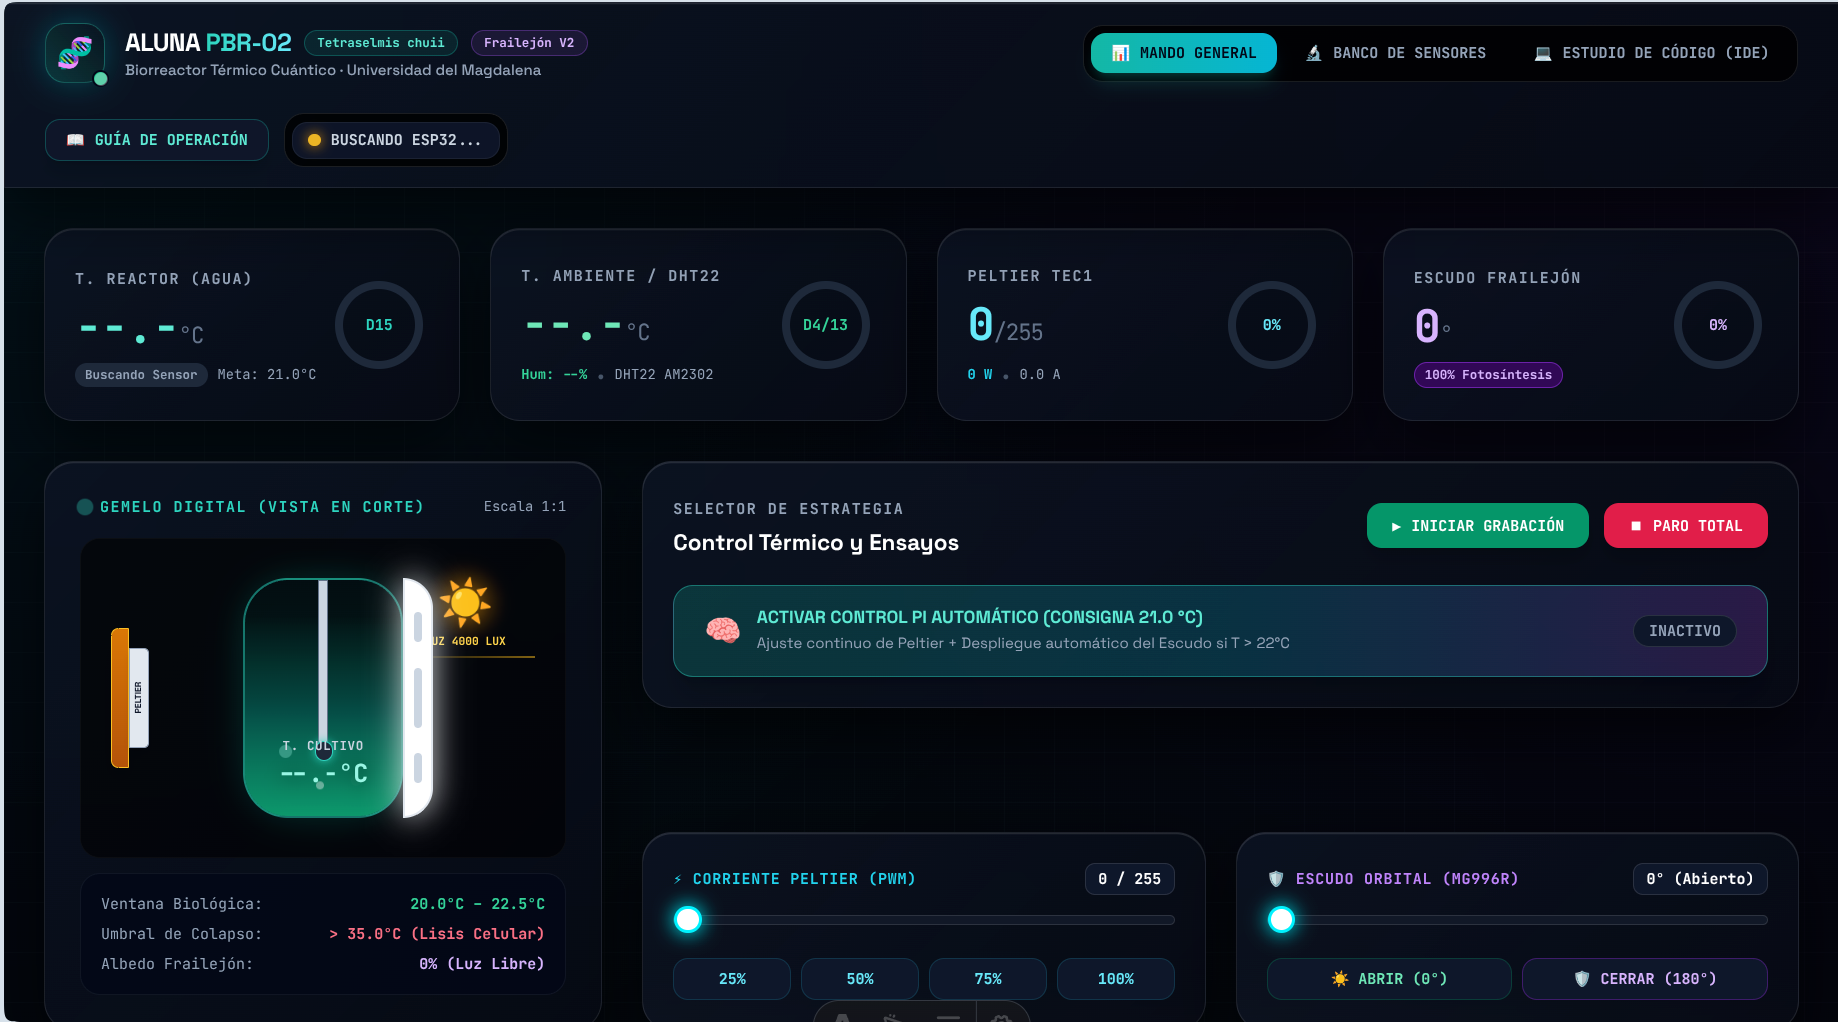
\includegraphics[width=0.92\textwidth]{imagenes/dashboard_telemetria.png}
    \caption{Captura real del Dashboard Web en operación mostrando telemetría en vivo y control PWM.}
    \label{fig:dashboard}
\end{figure}

El dashboard integra:
\begin{itemize}
    \item \textbf{Métricas Clave en Vivo:} Indicadores instantáneos de la temperatura del cultivo (Sensor 1 en D15), temperatura ambiental/disipador (Sensor 2 en D13), gradiente térmico $\Delta T$, porcentaje de modulación PWM y corriente estimada de la celda en amperios.
    \item \textbf{Gráficas Dinámicas ECharts:} Curvas temporales de alta resolución con ejes sincronizados, escalado dinámico y zoom interactivo que permiten observar la respuesta al escalón del reactor en tiempo real.
    \item \textbf{Consola de Comandos y Modo Manual:} Interruptores virtuales para conmutar entre control automático en lazo cerrado y control manual por PWM/ángulo servo para calibraciones de banco.
\end{itemize}
